% VOLUME OF RECTANGULAR PRISMS - WORKSHEET 0
\documentclass[12pt, letterpaper, fleqn]{article}

% ----------------------------------------------------------
% PACKAGES
% ----------------------------------------------------------
\usepackage{graphicx}
\usepackage{xcolor}
\usepackage[most]{tcolorbox}
\usepackage{amsmath, amssymb}
\usepackage{fancyhdr}
\usepackage[utf8]{inputenc}
\usepackage[T1]{fontenc}
\usepackage{enumitem}
\usepackage{geometry}
\usepackage{tikz}
\usepackage{needspace}
\usepackage{multicol}

\usetikzlibrary{arrows.meta, calc}

% ----------------------------------------------------------
% PAGE SETUP
% ----------------------------------------------------------
\usepackage{times}
\geometry{letterpaper, top=1.25in, bottom=1.25in, marginpar=0.5in}

% ----------------------------------------------------------
% HEADER / FOOTER
% ----------------------------------------------------------
\newcommand{\logowidth}{3cm}
\setlength{\headheight}{20pt}
\setlength{\footskip}{40pt}

\pagestyle{fancy}
\fancyhf{}
\fancyhead[C]{\small\bfseries Volume of Rectangular Prisms}
\fancyfoot[L]{\raisebox{2pt}{
\includegraphics[width=\logowidth]{kss.png}}}
\fancyfoot[C]{\thepage}
\fancyfoot[R]{6.18.0}

\renewcommand{\footrulewidth}{0.2pt}

% ----------------------------------------------------------
% HELPER MACROS
% ----------------------------------------------------------
\newcommand{\blank}{\underline{\hspace{2.2cm}}}
\newcommand{\blanklong}{\underline{\hspace{6.5cm}}}
\newcommand{\blankshorter}{\underline{\hspace{1.5cm}}}

% ----------------------------------------------------------
% DOCUMENT
% ----------------------------------------------------------
\begin{document}


% ==========================================================
% WORKSHEET 0: FOUNDATION
% ==========================================================
\pagestyle{fancy}
\fancyhf{}
\fancyhead[C]{\small\bfseries Volume of Rectangular Prisms --- Worksheet 0}
\fancyfoot[C]{\thepage}
\fancyfoot[R]{6.18.0}
\renewcommand{\footrulewidth}{0.2pt}

\textbf{Name:} \underline{\hspace{5cm}} \hfill \textbf{Date:} \underline{\hspace{3cm}}\\

\begin{tcolorbox}[colback=black!10]
    \large\textcolor{black}{\textbf{Volume of Rectangular Prisms (Foundation)}}
\end{tcolorbox}

\vspace{2mm}
\noindent
1. \textbf{Volume:} The amount of 3D space a solid shape occupies, measured in cubic units ($u^3$). \\
2. \textbf{Core Formulas:} \\
- $\text{Volume} = \text{length} \times \text{width} \times \text{height} = l \cdot w \cdot h$ \\
- $\text{Volume} = \text{Base Area} \times \text{height} = B \cdot h$, where $B = l \cdot w$. \\
3. \textbf{Fractional Side Lengths:} When edges are fractions, you can determine total capacity by finding how many fractional unit cubes layer inside the prism.

\vspace{3mm}

% --- 3D LAYERED PACKING SKETCH ---
\begin{center}
\begin{tikzpicture}[scale=0.9, every node/.style={transform shape}]
    % Draw outer prism wireframe
    \draw[thick, black] (0,0,0) -- (3,0,0) -- (3,2,0) -- (0,2,0) -- cycle;
    \draw[thick, black] (3,0,0) -- (3,0,-2) -- (3,2,-2) -- (3,2,0);
    \draw[thick, black] (0,2,0) -- (0,2,-2) -- (3,2,-2);
    \draw[thick, dashed, gray] (0,0,0) -- (0,0,-2) -- (3,0,-2);
    \draw[thick, dashed, gray] (0,0,-2) -- (0,2,-2);
    
    % Draw an illustrative unit layer line
    \draw[red, thick, dashed] (0,1,0) -- (3,1,0) -- (3,1,-2);
    
    % Dimensions
    \node[below] at (1.5,0,0) {Length ($l$)};
    \node[right] at (3,0,-1) {Width ($w$)};
    \node[left] at (0,1,0) {Height ($h$)};
    
    \node[anchor=west] at (4,1,-1) {$\mathbf{V = B \cdot h}$};
    \node[anchor=west, red] at (4,0.5,-1) {\small Area of Base ($B$) $= l \cdot w$};
\end{tikzpicture}
\end{center}

\vspace{2mm}

\begin{tcolorbox}[colback=white, colframe=black!25, boxrule=0.6pt, arc=4mm, left=6mm, right=6mm, top=4mm, bottom=4mm]
\textbf{Worked Example 1A: Fractional Edges}

\medskip
\noindent
Find the volume of a rectangular prism with length $3\frac{1}{2}$ in, width 2 in, and height $1\frac{1}{2}$ in.\\
\textbf{Solution:} Convert mixed numbers to improper fractions and multiply:
$$V = l \cdot w \cdot h = \frac{7}{2} \cdot \frac{2}{1} \cdot \frac{3}{2} = \frac{42}{4} = 10\frac{1}{2}\text{ in}^3.$$
\end{tcolorbox}

\vspace{3mm}

\begin{tcolorbox}[colback=white, colframe=black!25, boxrule=0.6pt, arc=4mm, left=6mm, right=6mm, top=4mm, bottom=4mm]
\textbf{Worked Example 1B: Unit Cube Packing Calculation}

\medskip
\noindent
\textbf{Problem:} How many small cubes with a side length of $\frac{1}{4}$ cm can pack inside a box with dimensions $1$ cm by $\frac{1}{2}$ cm by $\frac{3}{4}$ cm?

\medskip
\noindent
\textbf{Solution:} \\
1) Find the number of cubes along each edge dimension:\\
- Length: $1 \div \frac{1}{4} = 4\text{ cubes}$ \quad Width: $\frac{1}{2} \div \frac{1}{4} = 2\text{ cubes}$ \quad Height: $\frac{3}{4} \div \frac{1}{4} = 3\text{ cubes}$.\\
2) Multiply individual cube counts together: $\text{Total Cubes} = 4 \cdot 2 \cdot 3 = 24\text{ cubes}$.
\end{tcolorbox}

\newpage

\begin{tcolorbox}[colback=white, colframe=black, boxrule=1pt, arc=4mm, left=6mm, right=6mm, top=5mm, bottom=5mm]
\textbf{Deeper Thinking Problem 1: Unit Cube Packing}

\medskip
\noindent
\textbf{a)} A rectangular box has dimensions 3 cm by 2 cm by 1.5 cm. If we pack it completely with small cubes that have a side length of $\frac{1}{2}$ cm, how many small cubes will fit? Explain how this count matches the volume formula.
\vspace{3cm}

\noindent
\textbf{b)} A prism has a square base with sides of length $2.5$ meters. If its absolute volume is $25$ cubic meters, determine its height. Show your algebraic equation.
\vspace{2.5cm}
\end{tcolorbox}

\vspace{5mm}

\begin{tcolorbox}[colback=white, colframe=black, boxrule=1pt, arc=4mm, left=6mm, right=6mm, top=5mm, bottom=5mm]
\textbf{Deeper Thinking Problem 2: Scaling Prism Volume}

\medskip
\noindent
\textbf{a)} If you double all three core dimensions (length, width, and height) of a rectangular prism, what happens to its total volume? Test this by comparing a $2 \times 3 \times 4$ prism with its scaled counterpart.
\vspace{3cm}

\noindent
\textbf{b)} Find the exact volume of a geometric cube with side lengths of exactly $\frac{3}{4}$ foot. Express your answer as a fully simplified fraction.
\vspace{3cm}
\end{tcolorbox}

\newpage

\begin{tcolorbox}[colback=white, colframe=black, boxrule=1pt, arc=4mm, left=6mm, right=6mm, top=5mm, bottom=5mm]
\textbf{Deeper Thinking Problem 3: Volume and Capacity}

\medskip
\noindent
\textbf{a)} A fish tank is $2\frac{1}{2}$ feet long, $1\frac{1}{2}$ feet wide, and $1\frac{3}{4}$ feet tall. Find the volume of the tank. If 1 cubic foot $\approx 7.48$ gallons, how many gallons of water does it hold when filled?
\vspace{5cm}

\noindent
\textbf{b)} Two completely distinct prisms have the exact same volume of 120 cm$^3$. Prism A has a base area of 24 cm$^2$. Prism B has a base area of 40 cm$^2$. Calculate the height of each prism.
\vspace{5cm}

\noindent
\textbf{c)} A rectangular block of cheese measures $6\text{ cm} \times 4\text{ cm} \times 3\text{ cm}$. If you slice it entirely into smaller unit cubes with $1\text{ cm}$ edges, how many individual pieces do you obtain?
\vspace{5cm}
\end{tcolorbox}

\vspace{5mm}

\begin{tcolorbox}[colback=white, colframe=black, boxrule=1pt, arc=4mm, left=6mm, right=6mm, top=5mm, bottom=5mm]
\textbf{Deeper Thinking Problem 4: Real-World Volume Design}

\medskip
\noindent
\textbf{a)} A cargo truck area is 8 feet long, 6 feet wide, and 5 feet tall. Moving boxes are 2 feet long, 2 feet wide, and 1 foot tall each. How many boxes can stack perfectly inside the vehicle?
\vspace{5cm}

\noindent
\textbf{b)} A community swimming pool is 25 meters long, 10 meters wide, and 2 meters deep. If a supply hose fills the pool at a constant rate of 0.5 cubic meters of water per minute, how many hours will it take to fill completely?
\vspace{5cm}

\noindent
\textbf{c)} A rectangular fish tank is 3 feet long, 1.5 feet wide, and 2 feet tall. The tank is currently filled to only $\frac{3}{4}$ of its total volume with water. How many cubic feet of water are in the tank, and how many more cubic feet are needed to fill it completely?
\vspace{5cm}

\end{tcolorbox}


\end{document}
